\documentclass[times, twoside, watermark]{artigo}
\usepackage{blindtext}
\usepackage[utf8]{inputenc}
\citebrackets[]
\usepackage{indentfirst}
\renewcommand\refname{}
% \documentclass[article, 12pt, oneside, a4paper, twocolumn]{abntex2}
% \usepackage[left=3cm,top=3cm,right=2cm,bottom=2cm]{geometry}
% \usepackage[alf, abnt-etal-list=0, abnt-etal-cite=3]{abntex2cite}
% \usepackage{authblk}
% \usepackage{amsmath}
% \usepackage{amsfonts}
% \usepackage{amssymb}
% \usepackage{graphicx}
% \usepackage{verbatim}
% \usepackage{titlesec}

\begin{document}

% -------------------------------Titulo---------------------------------------------

\title{\Large {Desenvolvimento de firmware robusto e multiplataforma}}

\author[1]{Jonathan Gonzaga}
\author[2]{Orientador}

\affil[1]{Graduando em Engenharia de Computação, UNISAL São José - Campinas,
\href{mailto:jonathan.s.gonzaga@gmail.com}{jonathan.s.gonzaga@gmail.com}}
\affil[2]{Professor do UNISAL São José - Campinas,
\href{mailto:orientador@sj.unisal.br}{orientador@sj.unisal.br}}

\maketitle

% -------------------------------Resumo-Abstract-------------------------------------

\noindent\begin{abstract}
\textit{Resumo -} \normalfont{\textit{Este artigo apresenta técnicas e ferramentas 
para o desenvolvimento de firmware robusto e multiplataforma, com o intuito de 
minimizar bugs, permitir a implementação de testes unitários e incentivar o estudo de 
conceitos de Engenharia de software aplicados a sistemas embarcados.}}
\end {abstract}

\noindent\begin{keywords}
\textit{\textbf{Palavras-chave: }}\normalfont{\textit{sitemas embarcados, firmware, TDD, testes unitários}}
\end{keywords}

\noindent\begin{abstract}
\textit{Abstract - } \normalfont{\textit{This article presents techniques and tools 
for robust and multiplatform firmware development, in order to minimize bugs, allow 
the implementation of unit tests and encourage the study of software engineering 
concepts applied to embedded systems.}}
\end {abstract}
\noindent\begin{keywords}
\textit{\textbf{Keywords: }}\normalfont{\textit{embedded systems, firmware, TDD, unit tests}}
\end{keywords}
%\hfill\

% -------------------------------INTRODUÇÃO-----------------------------------------

%Esses dispositivos por si só já somam a maioria dos sistemas computacionais do mundo \cite{eetimes}. 
% Podemos chamar esses dispositivos de \textit{sistemas embarcados} (do inglês, embedded systems).

%É importante frisar que o ambiente no qual um sistema embarcado vai ser utilizado é 
% determinante não apenas para seu custo final, mas principalmente sua robustez e tolerância a falhas de hardware e software.

%Bugs em sistemas embarcados costumam ser críticos, pois espera-se que o produto funcione por anos sem apresentar problemas.

\section{INTRODUÇÃO }

Com o avanço da eletrônica e da computação, a miniaturização de circuitos integrados
e a redução de custos de fabricação, surgiram na indústria diversos dispositivos
eletrônicos com poder de processamento. 
A maioria desses dispositivos conta com processadores, memórias e periféricos
integrados, de forma que seu \textit{software} é destinado e \textit{embarcado} 
em uma aplicação específica. Sistemas dessa natureza são conhecidos como
\textit{sistemas embarcados}.

Produtos como eletrodomésticos, eletrônicos em geral, equipamentos médicos,
equipamentos de telecomunicações, ferramentas eletrônicas, sistemas de controle 
e automação e sistemas de tempo real em veículos são ou possuem sistemas embarcados
em sua concepção.

Devido ao alto nível de criticidade de alguns sistemas embarcados, é esperado que o
\textit{software} executado neles seja altamente confiável e com o mínimo de
\textit{bugs} possível. 
A realidade da indústria de eletrônicos mostra que essa afirmação nem sempre é 
verdadeira.

Erros e falhas de \textit{software} são um problema em diversas áreas da tecnologia. 
Desde vulnerabilidades que facilitam a ação de \textit{hackers} em redes sociais,
falhas em \textit{smartphones} que causam travamento do sistema operacional a
inconsistências no acionamento de sistemas de freios que causam acidentes em
veículos. Esse último caso é ainda mais grave, pois o sistema lida diretamente com
vidas humanas. 

Especialistas em desenvolvimento de \textit{firmware} e \textit{software} embarcado, 
como Jack Ganssle, James W. Grenning e Jacob Beningo, dedicaram-se a criar 
literatura de qualidade, escrevendo livros e artigos com técnicas e 
metodologias de desenvolvimento de \textit{software}. 
Alguns títulos relevantes são: \textit{Test-Driven development for Embedded C}
\cite{tddembeddedc}, 
\textit{The Art of Designing Embedded Systems}\cite{ganssle2008art} e
\textit{Reusable Firmware Development}\cite{beningo2017reusable}. 
A partir dessas obras muito se tem discutido sobre como criar sistemas mais seguros, 
com menor probabilidade de erros e menos suscetíveis a má utilização por parte do usuário.

No processo de desenvolvimento de \textit{software}, o custo de uma alteração no 
código tende a ficar maior conforme  as etapas do desenvolvimento avançam, por isso 
o custo de um \textit{bug} encontrado em campo após o produto ser lançado, é muito 
maior que o custo do mesmo sendo encontrado ainda na fase de desenvolvimento\cite{firmwarecost}.
Esse cenário por si só já mostra a necessidade de se detectar problemas nas fases iniciais do projeto.

\textit{Software} para sistemas embarcados muitas vezes é difícil de ser testado e 
validado, extremamente dependente da plataforma de \textit{hardware target}, e 
tende a demonstrar problemas de integração com outras
partes do sistema após a inserção de novas funcionalidades. 
Devido a limitação de recursos e a extrema dependência do \textit{hardware}, testes 
automatizados não são realizados, o que acaba prejudicando a qualidade do código.

Metodologias e conceitos como \textit{TDD (Test-Driven development)}, pirâmide de 
testes e \textit{SOLID}, são historicamente e erroneamente atribuídos apenas
aos \textit{softwares} de "alto nível", como \textit{web} ou 
\textit{mobile} por exemplo, afastando os desenvolvedores de \textit{software} 
embarcado desses conceitos e da utilização de abstrações mais inteligentes. 

Com essas dificuldades em mente, percebe-se a necessidade de se estimular as boas 
práticas de desenvolvimento de \textit{software} embarcado, a utilização de testes 
automatizados e independentes do \textit{hardware}, e o estudo de conceitos de 
engenharia de \textit{software} que auxiliem na
redução de \textit{bugs} e consequentemente, redução de custos do projeto e aumento 
da qualidade do código gerado. \hfill\\



% ----------------------REFERENCIAL TEÓRICO-----------------------------------

\section{REFERENCIAL TEÓRICO}

\subsection{Firmware}\hfill\\

\textit{Firmware} é um tipo específico de \textit{software} executado diretamente
num circuito integrado (ou \textit{chip}). 
Não necessita de outros programas para ser executado (como sistemas operacionais),
além de servir a um propósito único. 
Em outras palavras, é o \textit{software} executado em um sistema
embarcado\cite{ganssle2004firmware}.

Devido a limitações de tamanho e recursos desse tipo de sistema, 
o \textit{firmware} precisa manipular o \textit{hardware} diretamente e toda a sua
 arquitetura costuma ser voltada a eventos do mundo externo.

Diferente de sistemas computacionais mais complexos e com alto nível de abstração,
onde geralmente o \textit{kernel} do sistema operacional é modularizado e abstrai
o acesso a dispositivos de \textit{hardware}\cite{tanenbaum2015modern},
num sistema embarcado o \textit{firmware} é responsável pela gerência dos recursos 
e eventos de \textit{hardware} (interrupções e exceções do processador) e também
pelo código da aplicação (regras de negócio, interface com usuário e demais especificidades).

Muitas vezes ele faz parte de um sistema computacional maior,
por exemplo, computadores \textit{desktop} possuem circuitos integrados para 
aplicações específicas, como a \textit{BIOS} (\textit{Basic Input/Output System}),
que trata-se de um mecanismo responsável pela inicialização dos
componentes de \textit{hardware} do computador. \cite{terzicbasic}

Algumas literaturas não fazem distinção entres os termos \textit{firmware} e 
\textit{software embarcado}, sendo ambos utilizados como sinônimos. Por uma
questão de organização, será realizada uma distinção entre
esses termos: \textit{firmware} é o \textit{software} executado num circuito 
integrado comumente escrito em linguagem \textit{C, C++}, ou mesmo \textit{Assembly}. 
Já o \textit{software embarcado} possui características de alta abstração, 
sendo uma aplicação (um processo rodando num sistema operacional, 
geralmente baseado em \textit{GNU/Linux})\cite{simmonds2015mastering} porém executado 
em dispositivos de propósito específico (como roteadores e terminais de autoatendimento). 
Pode ser escrito em linguagens de programação como \textit{C, C++, Rust, Go, Python} entre outras.

Em um sistema embarcado executando um \textit{firmware}, o cérebro por trás de todo o 
processamento é um componente chamado \textit{microcontrolador}.


\subsection{Microcontroladores}\hfill\\

Microcontroladores são processadores de pequeno porte contendo \textit{CPU}, 
memórias (\textit{RAM} e \textit{FLASH}) e demais
recursos atrelados no mesmo encapsulamento ou \textit{SoC (System on Chip)}.
Esses recursos são denominados periféricos, e são inclusos no \textit{chip} 
com o intuito de tornar possível o interfaceamento entre a \textit{CPU} 
e o mundo externo, permitir a comunicação com outros dispositivos e 
aquisitar dados para posterior processamento através dos pinos físicos do componente.

Os recursos mais comuns são as interfaces de comunicação 
serial (\textit{USART, I2C, SPI}), conversores analógico-digital e digital-analógico 
(\textit{ADC} e \textit{DAC}), temporizadores/contadores (\textit{TIMERS}) e 
interface de pinos (\textit{GPIO}).

Com tamanho e custo reduzidos em comparação ao microprocessadores,
os microcontroladores tornam-se economicamente viáveis, além da
escolha óbvia, para controlar digitalmente dispositivos e processos\cite{gridling2007introduction}.

\subsection{Testes de software}\hfill\\

Testes de \textit{software} são procedimentos pelos quais o código fonte de um
\textit{software} é submetido afim de validar seu comportamento mediante
os requisitos pelos quais foi projetado.

Existem diversos tipos de testes de \textit{software}, cada um responsável por 
testar partes e situações diferentes. A chamada \textit{Pirâmide de testes}
\cite{contan2018test} foi concebida com o intuito de seguimentar os testes em três 
grandes níveis:

\begin{itemize}
\item \textit{Testes end-to-end} - simulam a aplicação final
\item \textit{Testes de integração} - testa a integração entre testes de unidade
\item \textit{Testes unitários} - testes de unidade, verificam a menor unidade de código testável
\end{itemize}

Apenas o último nível, os testes unitários, serão abordados nesse documento.

\subsection{Testes unitários}\hfill\\

Testes unitários são a base dos testes de \textit{software}. Na \textit{Pirâmide de 
testes} encontram-se no nível mais baixo, o que indica que são 
o tipo mais barato, mas também os mais fáceis de se 
implementar\cite{contan2018test}.

Como seu nome sugere, são testes de \textit{unidade}, onde é possível testar a 
menor unidade testável do código (sejam funções, classes ou módulos).

\subsection{TDD - Test-Driven development}\hfill\\

\textit{Test-Driven development} (ou \textit{Desenvolvimento orientado a testes}) é uma técnica
incremental de construção de \textit{software}. 
Nessa técnica, nenhum código de produção é escrito sem que primeiro seja escrito um 
teste unitário que falhe na primeira execução. 

Ao contrário da prática comum de desenvolvimento de \textit{software}, onde primeiro é desenvolvido o
código de produção e só depois os testes, no TDD
o desenvolvedor expressa o comportamento desejado do código em um teste. 
O teste é executado e falha. Só então ele escreve o código de produção, fazendo o teste passar.
A automação de testes é a chave para o \textit{TDD}. Os testes são pequenos e automatizados.
A cada nova funcionalidade implementada, novos testes unitários são escritos, 
seguidos imediatamente por um código de produção que satisfaça aqueles testes. 

Conforme o código de produção cresce, também crescem em conjunto os testes unitários, 
que são ativos tão valiosos quanto o próprio código de produção. 
A cada mudança de código, o conjunto de testes é executado, verificando a funcionalidade da nova
implementação, mas também a compatibilidade com o código já existente\cite{tddembeddedc}.

% ----------------------METODOLOGIA-----------------------------------
\section{METODOLOGIA}\hfill\

A metodologia utilizada para o desenvolvimento do projeto segue a técnica de \textit{TDD} descrita anteriormente. 
Um esquema simplificado pode ser visto na figura a seguir:\hfill\

\begin{figure}[H]
    \centering
    \caption{Esquema simplificado do TDD}
    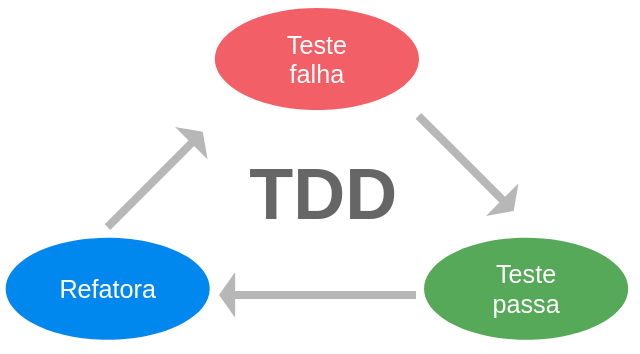
\includegraphics[width=0.95\linewidth]{images/tdd.png}
    \caption*{\newline\textbf{Fonte:} acervo do autor}
\end{figure}

Três grande etapas são necessárias: \textit{Teste falha}, \textit{Teste passa}
e \textit{Refatora}. Na primeira, são escritos apenas os testes unitários, com base 
nos requisitos do projeto, porém sem nenhum código de produção ainda, o que 
obviamente fará com que os testes falhem após a execução.

Logo após, são escritos apenas os trechos de código necessários para que aqueles 
testes passem e nada mais.

Na última etapa, o código passará pelo processo de \textit{refatoração}, onde serão 
eliminados possíveis erros, duplicidade, e será formatado de acordo com o padrão 
requisitado.

Nas três etapas serão utilizadas ferramentas e mecanismos de software para auxílio
na implementação dos testes, execução e automatização de processos.

\subsection{MATERIAIS E MÉTODOS}
%Reseta o contador de subsection
% \setcounter{section}{-1}\stepcounter{section}

\subsubsection{Software - Ceedling}\hfill\\

\textit{Ceedling} é um \textit{build system} (sistema de construção de 
\textit{software}) para projetos escritos em linguagem C.
É uma espécie de extensão do sistema de construção \textit{Rake (make-ish)} do \textit{Ruby}.
O \textit{Ceedling} é voltado principalmente para o 
Desenvolvimento Orientado a Testes (TDD) em C e é projetado para reunir as ferramentas \textit{CMock},
\textit{Unity} e \textit{CException} - três outros projetos de código aberto 
que auxiliam na dinâmica de testes automatizados\cite{gomes2016uttos}.


\subsubsection{Software - FreeRTOS}\hfill\\

\textit{FreeRTOS} é um \textit{kernel} de tempo real, 
ou um sistema operacional de tempo real (\textit{Real-Time Operating System}) 
para dispositivos embarcados. Foi desenvolvido para ser pequeno, simples e portável. 
Seu \textit{kernel} é composto por apenas 3 arquivos em linguagem C. 
O \textit{FreeRTOS} permite a fácil implementação de multitarefa preemptiva 
ou não preemptiva com diversos níveis de prioridade de tarefas\cite{zhu2016understanding}.


% ----------------------DESENVOLVIMENTO-----------------------------------

\section{DESENVOLVIMENTO}

%Reseta o contador de subsections
% \setcounter{section}{-1}\stepcounter{section}
O processo de desenvolvimento do projeto seguiu o padrão especificado anteriormente,
juntamente com algumas regras e boas práticas:

\begin{itemize}
\item \textit{Clean Code} (Código limpo) - o código precisa ser de fácil 
entendimento\cite{martin2009clean}
\item \textit{KISS (Keep it simple stupid)} - as soluções implementadas precisam ser 
simples\cite{martin2018clean}
\item \textit{SOLID principles} - seguir os padrões do \textit{SOLID}
\cite{martin2002agile}
\end{itemize}

\subsection{Arquitetura de \textit{software} do sistema}\hfill\\
Abaixo pode-se ver os componentes de \textit{software} separados por nível de abstração:\hfill\\

\begin{figure}[H]
    \centering
    \caption{Arquitetura de software do projeto}
    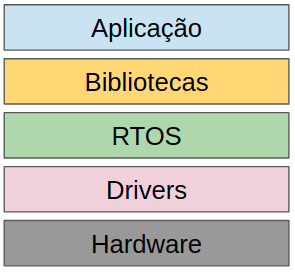
\includegraphics[width=0.7\linewidth]{images/arch.png}
    \caption*{\newline\textbf{Fonte:} acervo do autor}
\end{figure}

\subsection{Dual-targeting: compilando para duas arquiteturas}\hfill\\

Um dos pilares do desenvolvimento de \textit{software} multiplataforma é a abstração.
Utilizar interfaces bem definidas apartir de \textit{header files}, variando apenas
a implementação dessas interfaces nos \textit{source files}.

\subsection{Camadas de abstração - drivers e RTOS}\hfill\\

Para se escrever código portável é extremamente necessário a não dependência de 
\textit{hardware}, \textit{RTOS - (Real Time Operating Systems)} e demais bibliotecas

\subsection{Testes unitários}\hfill\\

Para escrever testes unitários, é necessário a utilização de um \textit{framework}

% ----------------------CONCLUSÃO-----------------------------------

\section{CONCLUSÃO}\hfill\\
Conclui-se que 


% \section{REFERÊNCIAS}
\bibliography{artigo}

\end{document}
